\section{Methodology}

The goals of this project would be an Automated Testing Framework for GraalVM's optimization DSL. This would represent another tool that the 
developers of GraalVM could use to provide a \emph{certificate} towards their implementation code. In order to assist in verifying the optimization 
phase, the tool would need to be able to determine whether:

\begin{enumerate}
    \item The optimization phase are obviously false;
    
          This would require the tool to generate obvious counterexamples via Quickcheck (See \ref{sec:Quickcheck}) or Nitpick (See \ref{sec:Nitpick}).

    \item The optimization phase are obviously true;
    
          This would require the tool to verify that Sledgehammer (See \ref{sec:Quickcheck}) are able to provide proof obligations for the 
          optimization phase \textbf{without} defining proof tactics.

    \item The optimization phase would require manual proving by \emph{"proof experts"}.
          
          This means that the optimization is non-trivial: Isabelle are not able to find an obvious counterexample, and proving would require 
          additional tactics or subgoals to be defined.

\end{enumerate}

Furthermore, there are several key requirements for the system that needs to be satisfied:

\begin{enumerate}
      \item Developers of GraalVM needs to be able to integrate this easily on their test suite;
      \item Developers of GraalVM can easily use this without understanding Isabelle;
      \item \emph{If possible}, the system doesn't require enormous computing resources locally.
\end{enumerate}

In order to do this, it would require the project to explore whether its even possible to utilize Isabelle as the core system of the framework. 
Hence, understanding Isabelle's implementation are crucial in order to achieve the goals of this project. At a glance, there are three options 
to the project:

\begin{itemize}
    \item Utilize \mono{Isabelle Server} - \mono{Client} interactions (See \ref{sec:IsabelleServer});
    \item Extend \mono{Isabelle/Scala} (See \ref{sec:IsabelleScala});
    \item Create an Interpreter for GraalVM's optimization DSL (See \ref{sec:DSLInterpreter}).
\end{itemize}

\begin{figure}[h]
      \centering
      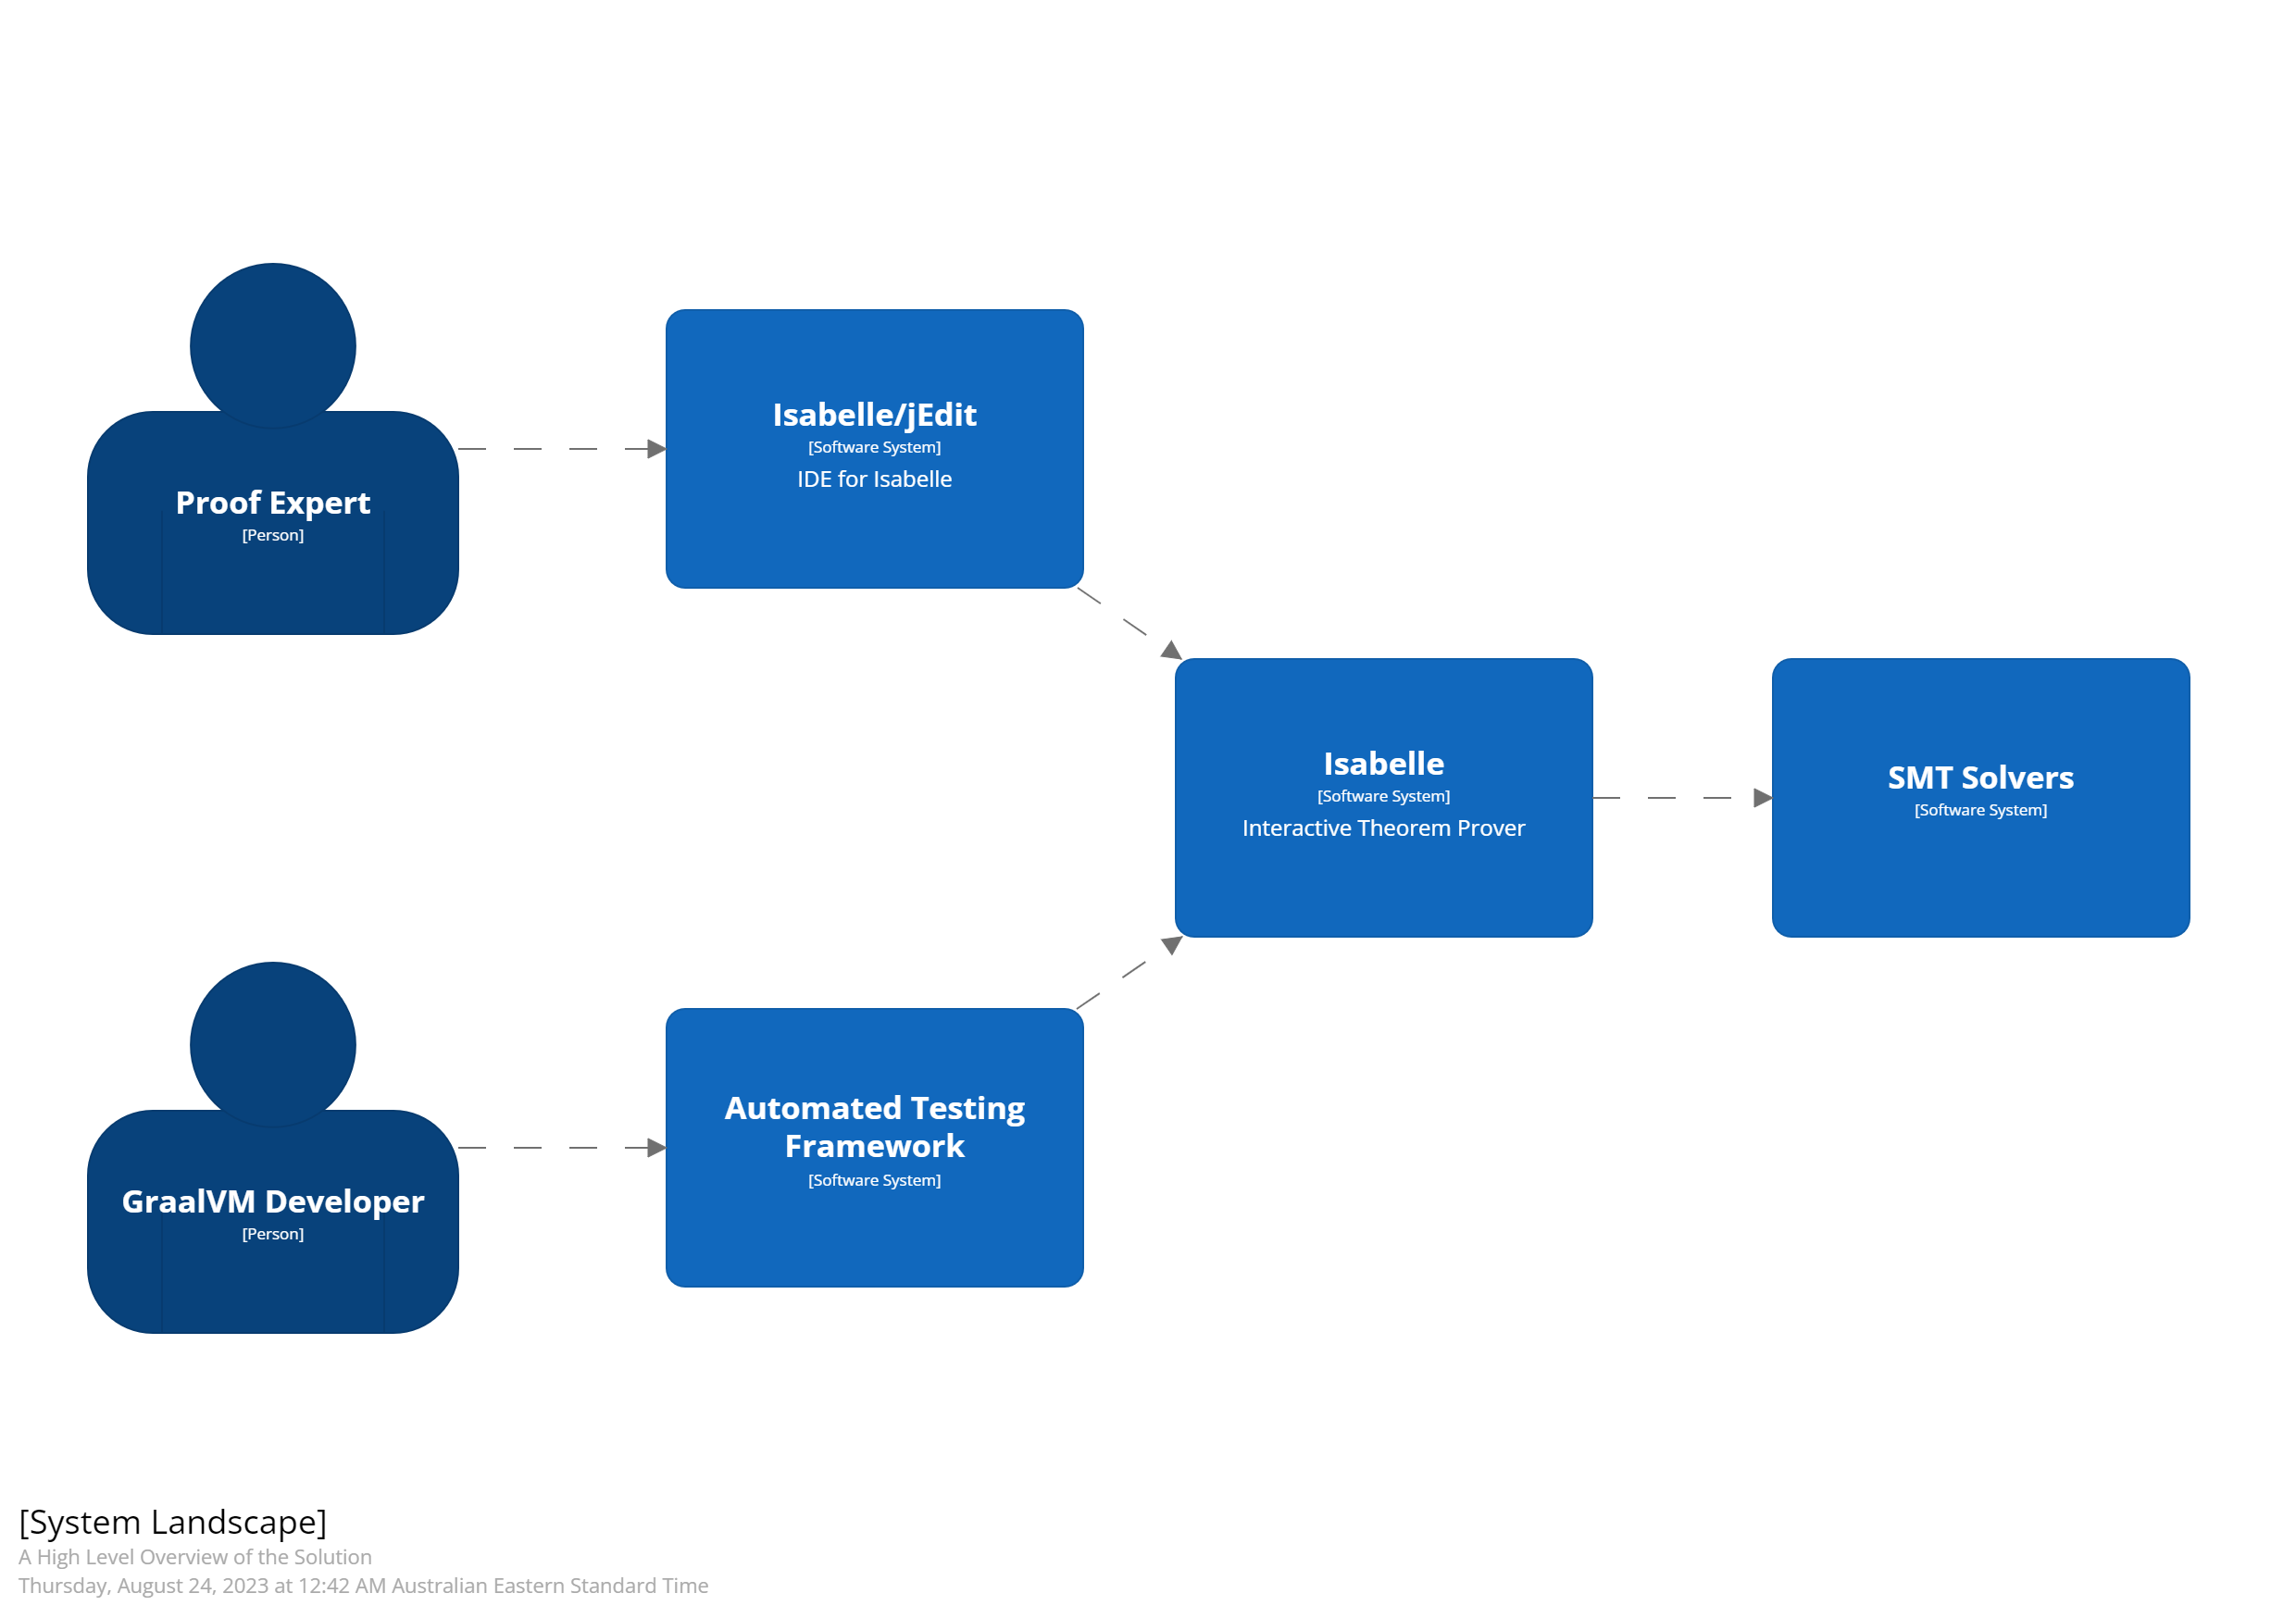
\includegraphics[width=0.6\textwidth]{structurizr-1-framework_overview_1.png}
      \caption{Proposed Solution}
      \label{fig:SystemLandscape}
\end{figure}

Figure \ref{fig:SystemLandscape} depicts the overview of the proposed solution's system landscape. In theory, it would utilize Isabelle in a similar 
manner as Isabelle/jEdit \cite{isabelleSystem}. Therefore, it should be able to use the the same Isabelle functionalities as Isabelle/jEdit does.

\pagebreak

\subsection{Isabelle System Overview}
\label{sec:IsabelleSystemOverview}

\begin{figure}[h]
      \centering
      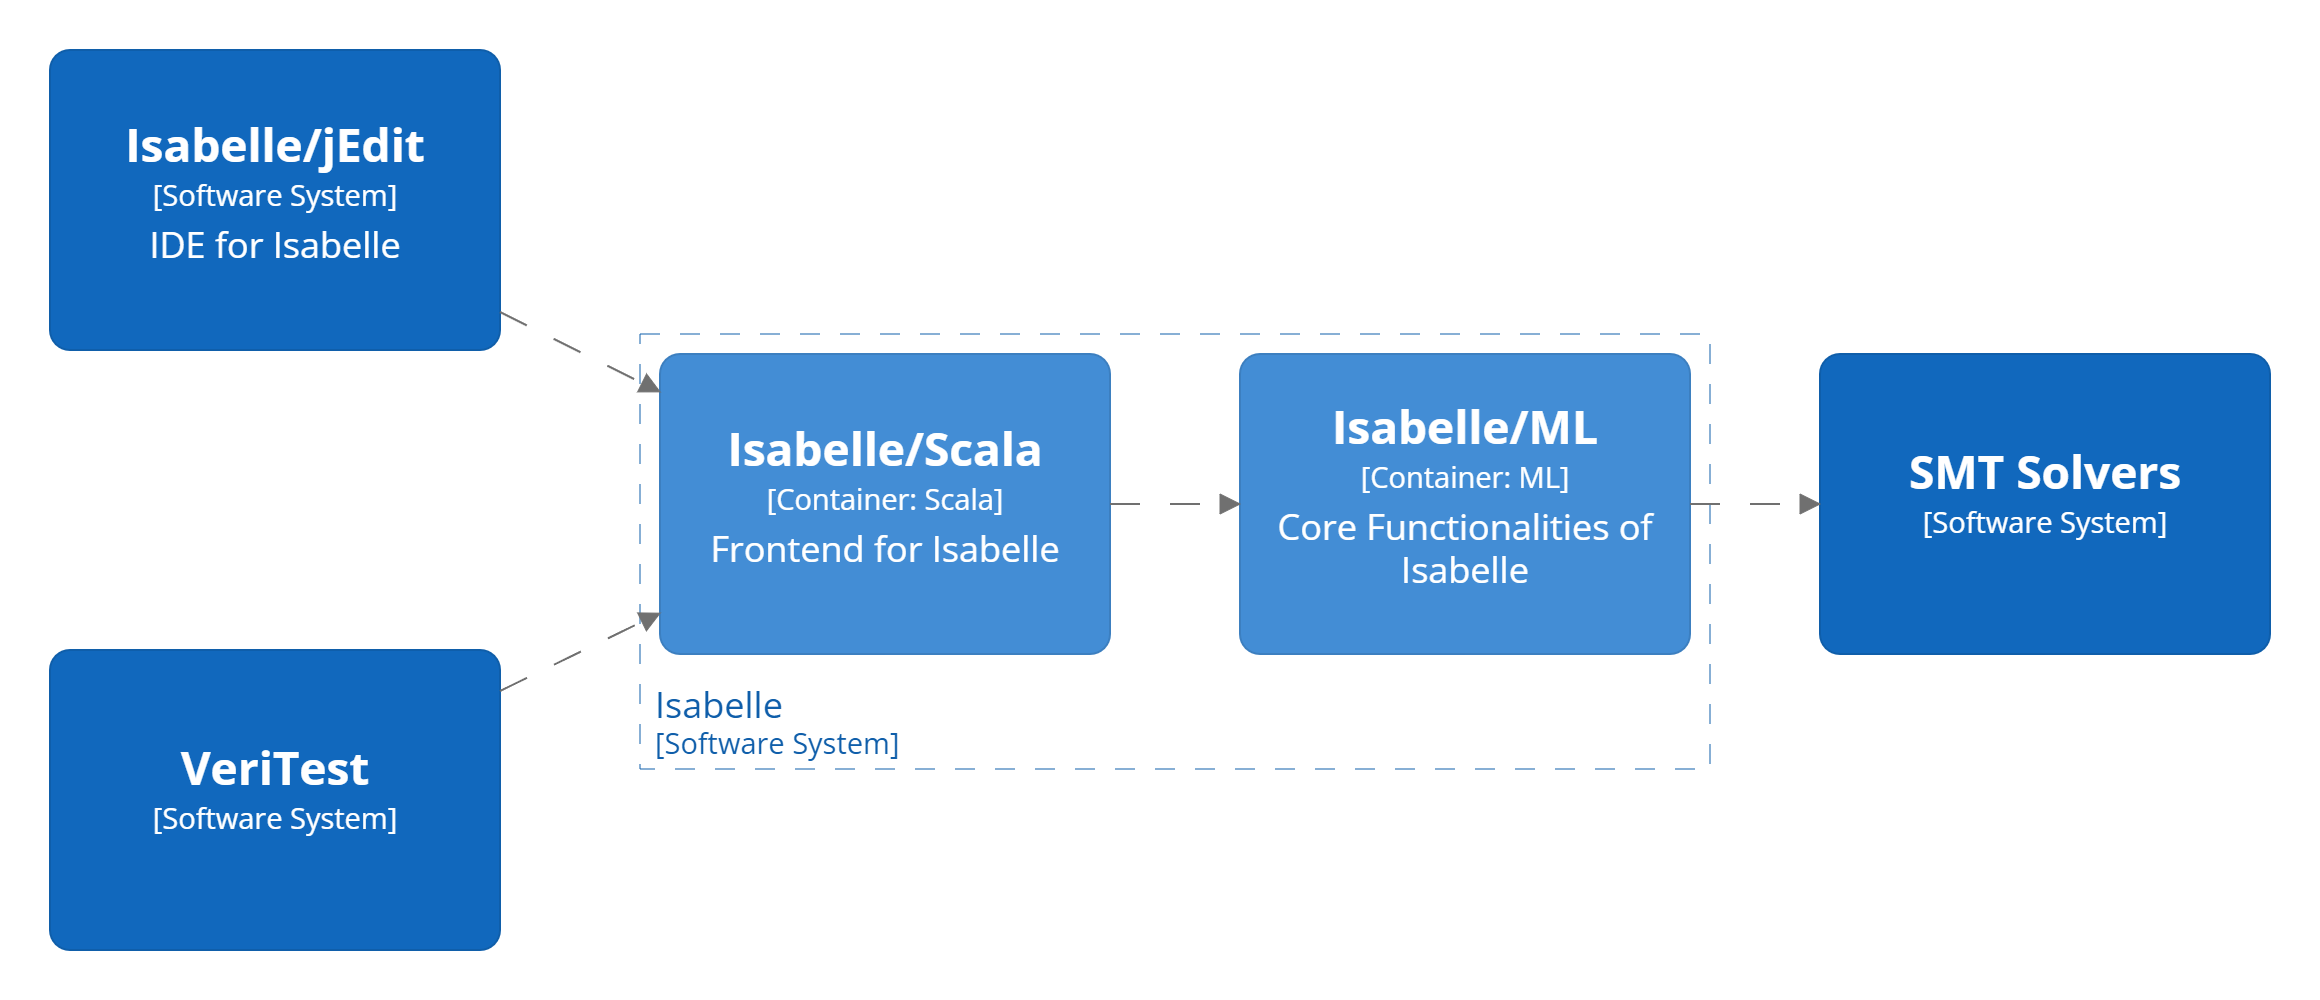
\includegraphics[width=0.6\textwidth]{structurizr-1-isabelle_overview_1.png}
      \caption{Isabelle System Overview}
      \label{fig:IsabelleSystem}
\end{figure}

Isabelle are made up of two significant components: Isabelle/ML and Isabelle/Scala \cite[Ch. 5]{isabelleSystem}. Isabelle/ML acts as the core 
functionality of Isabelle, harboring all the tools needed for proving theorems. Isabelle/Scala acts as the system infrastructure for Isabelle/ML 
-- hiding all the implementation details of Isabelle/ML.

\subsection{Utilizing Isabelle Server}
\label{sec:IsabelleServer}

\begin{figure}[h]
      \centering
      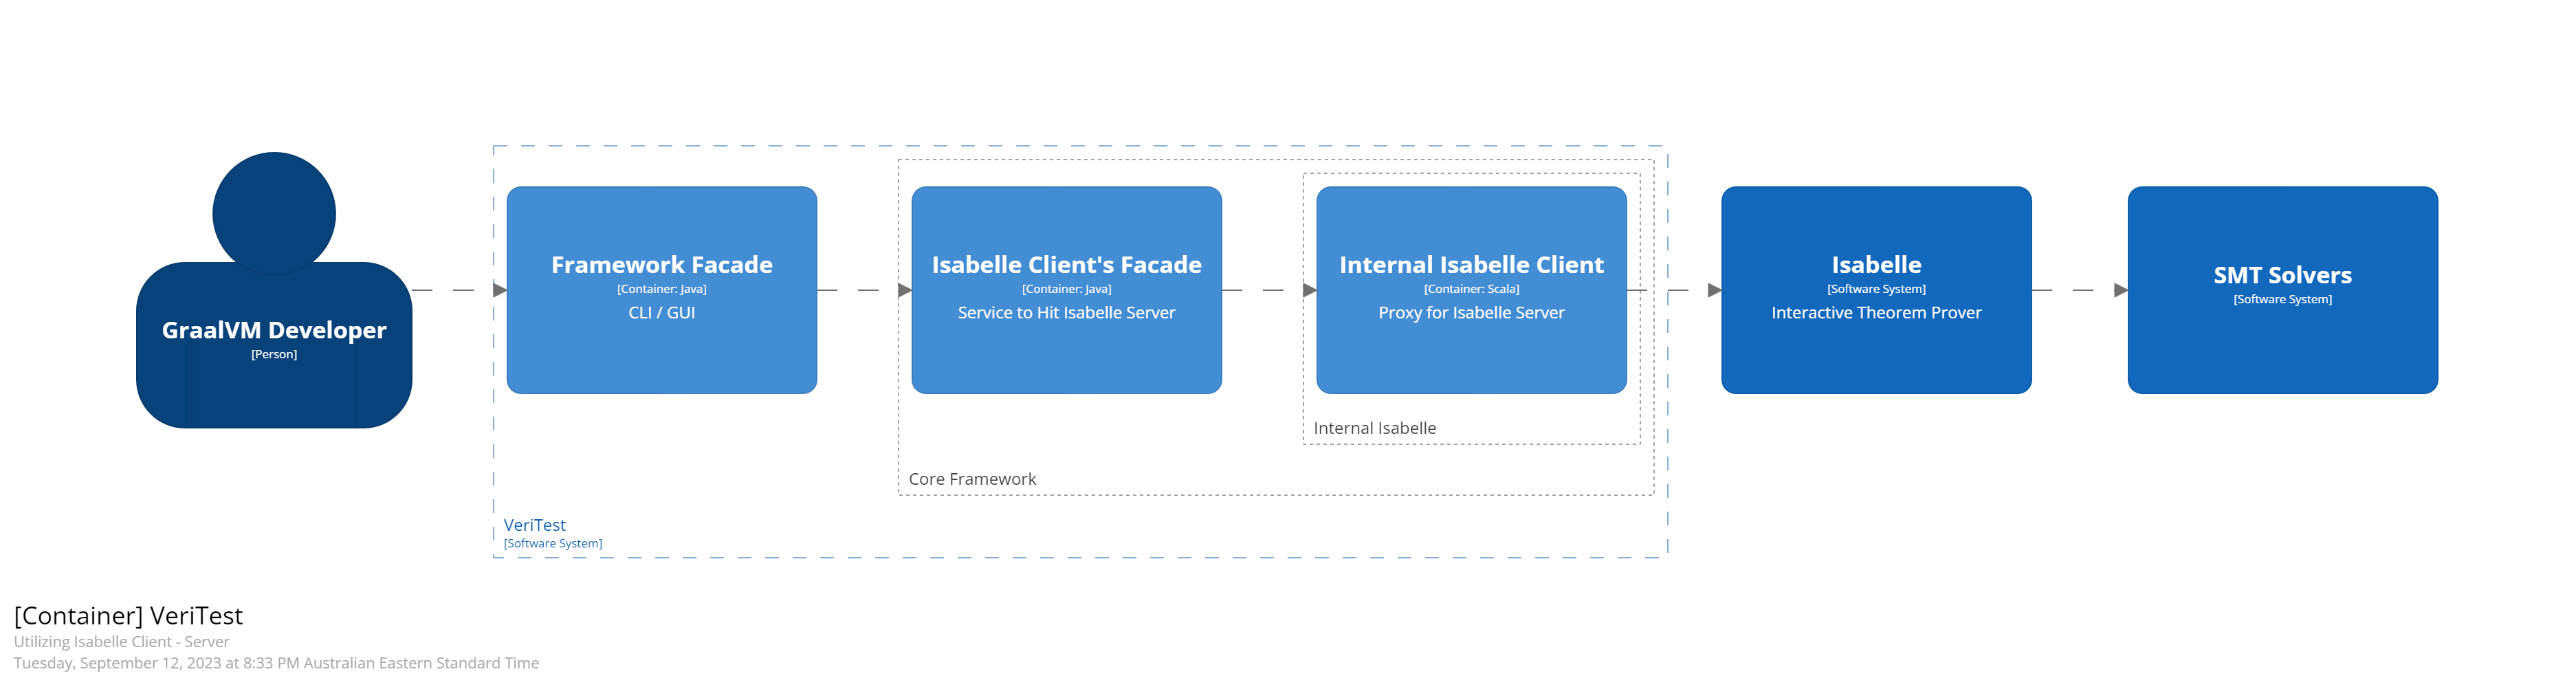
\includegraphics[width=0.8\textwidth]{structurizr-1-isabelle_client_server_1.png}
      \caption{Utilizing Isabelle Client - Server interaction}
      \label{fig:IsabelleServer}
\end{figure}

Isabelle Server acts as the core Isabelle process that allows theorems and all the required facts to be loaded up and processed by Isabelle/ML
\cite[Ch. 4]{isabelleSystem}. Interactions to Isabelle/Server would require duplex socket connection over TCP \cite[Ch. 4.2]{isabelleSystem}. 
To simplify the communication between the framework and Isabelle/Server, we utilize Isabelle Client \cite[Ch. 4.1.2]{isabelleSystem} -- a proxy 
for Isabelle/Server that handles all the communication protocols of Isabelle/Server.

Isabelle Server are able to load theorems and process requests in parallel \cite[Ch. 4.2.6]{isabelleSystem}. As such, this solution would be ideal 
for the project, as it would allow the framework to offload the computing resources of loading and processing optimization proofs on external sites.
However, it would require a \emph{Facade} that's able to demultiplex asynchronous messages on Isabelle Client (See Fig. \ref{fig:IsabelleServer}). 
Furthermore, the full capabilities of Isabelle Server needs to be explored in order to implement this option.

\subsection{Extending Isabelle/Scala}
\label{sec:IsabelleScala}

\begin{figure}[h]
      \centering
      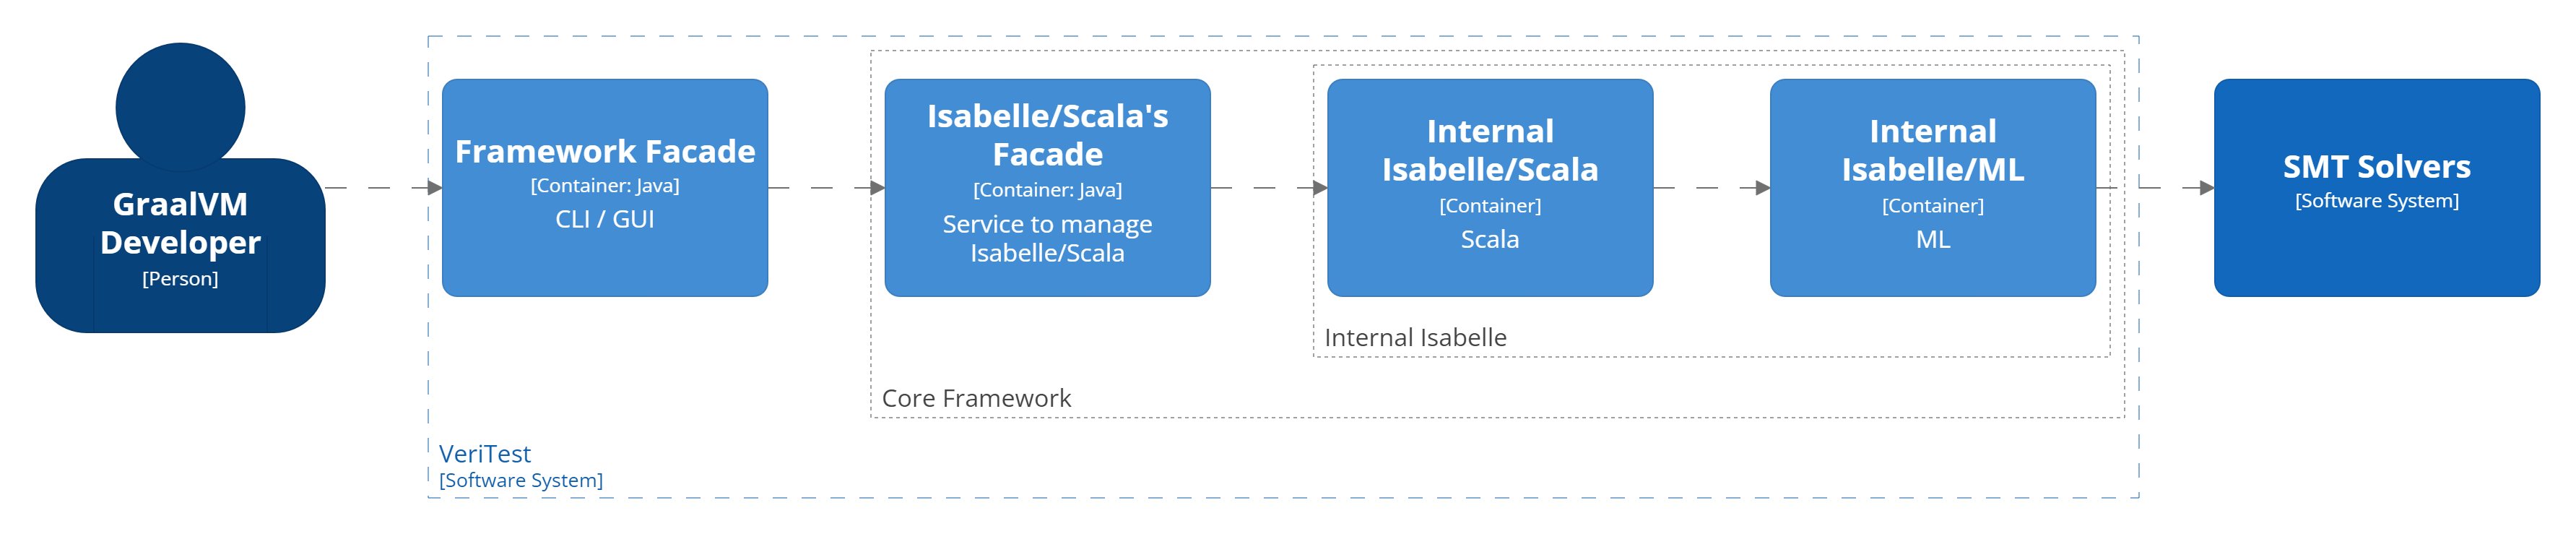
\includegraphics[width=0.8\textwidth]{structurizr-1-isabelle_scala_1.png}
      \caption{Extending Isabelle/Scala}
      \label{fig:IsabelleScala}
\end{figure}

Isabelle can be extended by accessing Isabelle/Scala functions \cite[Ch. 5]{isabelleSystem}. Extending Isabelle/Scala would require the framework 
to utilize Isablle's Scala compiler \cite[Ch. 5.1.4]{isabelleSystem}. Consequently, it means that Isabelle/ML would be bundled with Isabelle/Scala. 
As such, this option would be able to utilize all the functionalities of Isabelle. Figure \ref{fig:IsabelleScala} depicts the proposed solution for 
this option.

However, the full complexity of Isabelle/Scala are an unknown. Currently Isabelle/Scala is not well documented, and would require much of the 
project's timeline to understand Isabelle/Scala. Furthermore, extending Isabelle/Scala \emph{could} mean that the framework would take up 
much of the computing resources to execute Isabelle/ML functions locally.

\subsection{Interpreter for DSL}
\label{sec:DSLInterpreter}

Building an interpreter for GraalVM's optimization DSL acts as a last resort to the project. In order to implement this, it would require significant 
amount of time to rework the DSL into the framework, and desigining tools similar to Quickcheck (See \ref{sec:Quickcheck}) in order to satisfy the 
system requirements. Reinventing the wheel would not be productive for the project, and it would result in a tool that is far inferior to Isabelle.
Therefore, this option should be avoided \emph{if possible}.